\documentclass[11pt,a4paper]{article}

\usepackage[top=1.25cm,bottom=1.15cm,left=1.15cm,right=1.15cm]{geometry}
\usepackage[T1]{fontenc}
\usepackage[utf8]{inputenc}
\usepackage{lmodern}
\usepackage{enumitem}
\usepackage[hidelinks]{hyperref}
\usepackage{xcolor}
\usepackage{titlesec}
\usepackage{microtype}
\usepackage{tabularx}
\usepackage{fontawesome5}
\usepackage{pagecolor}

\usepackage{helvet}
\renewcommand{\familydefault}{\sfdefault}

\pagestyle{empty}
\setlength{\parindent}{0pt}
\setlength{\parskip}{4pt}
\hfuzz=3pt
\setlist[itemize]{leftmargin=*, topsep=1pt, itemsep=1pt}

\definecolor{heading}{RGB}{25,25,25}
\definecolor{timelineblue}{RGB}{30,58,95}
\definecolor{timelinegray}{RGB}{80,80,80}

\definecolor{pagebg}{RGB}{241,241,244}
\definecolor{cardbg}{RGB}{255,255,255}
\pagecolor{pagebg}

\titleformat{\section}{\large\bfseries\color{heading}}{}{0pt}{}[\vspace{-4pt}\hrule\vspace{4pt}]

\usepackage{tikz}
\usetikzlibrary{positioning}

\newcommand{\projectcard}[4]{
\noindent
\begin{tikzpicture}
\node[
    text width=0.96\textwidth,
    fill=cardbg,
    draw=timelinegray!25,
    rounded corners=3pt,
    inner sep=6pt,
    align=left
] (box) {
\begin{tabularx}{0.96\textwidth}{@{}p{1.05cm}@{\hspace{0.3cm}}X@{}}
{\LARGE\color{timelineblue}#1} &
\begin{minipage}[t]{\linewidth}
{\normalsize\textbf{#2}}\\[2pt]
{\footnotesize #3}
\end{minipage}
\end{tabularx}
};

\node[
    anchor=south east,
    fill=gray!8,
    draw=timelinegray!20,
    rounded corners=2pt,
    inner xsep=5pt,
    inner ysep=2pt
] at ([xshift=-6pt,yshift=6pt]box.south east) {
    {\tiny #4}
};

\end{tikzpicture}
\vspace{3pt}
}

\begin{document}

\noindent\rlap{%
\begin{tikzpicture}[remember picture,overlay]
\node[
    anchor=south,
    yshift=0.35cm,
    text width=17.9cm,
    fill=cardbg,
    draw=timelineblue!35,
    rounded corners=5pt,
    inner sep=8pt
] at (current page.south) {
{\scriptsize
{\small\bfseries\color{timelineblue}
\faCogs\ SKILLS
}

{\color{timelineblue!40}\rule{\linewidth}{0.4pt}}

\vspace{3pt}
\begin{tabularx}{17.7cm}{@{}X X X X X@{}}
\textbf{\color{timelineblue}Android} &
\textbf{\color{timelineblue}Architecture} &
\textbf{\color{timelineblue}Platform} &
\textbf{\color{timelineblue}Engineering} &
\textbf{\color{timelineblue}Backend \& Systems} \\[3pt]

Kotlin &
MVVM &
Android Enterprise &
Gradle &
Python / FastAPI \\

Android SDK &
Clean Architecture &
Device Owner &
CI/CD &
PowerShell \\

Coroutines / Flow &
Reusable Components &
Device Policy Manager &
Automated Testing &
Active Directory \\

REST APIs &
Local-first Systems &
Kiosk / Device Mgmt &
Release Packaging &
Kerberos / SMB / GPO \\
\end{tabularx}
}
};
\end{tikzpicture}%
}
\begin{tabularx}{\textwidth}{@{}X r@{}}
    {\LARGE \textbf{Daniele Della Cioppa}} &
    \href{https://github.com/danieledellacioppa}{\Large \faGithub\ GitHub} \\
    {\normalsize Android Software Engineer --- Kotlin, Mobile Platforms \& Distributed Systems} &
    \href{https://www.linkedin.com/in/daniele-della-cioppa-41b062115/}{\Large \faLinkedin\ LinkedIn} \\
    London, UK & \\
\end{tabularx}

\smallskip

\footnotesize{
Android Software Engineer specialising in Kotlin and maintainable mobile platform development. I build Android applications and reusable platform capabilities with MVVM, Clean Architecture, coroutines, Flow, REST API integration and local-first patterns for managed device environments. My experience covers distributed Android device systems, digital signage, controlled application delivery, Android Enterprise, Device Owner workflows and remote device management where reliability, testability and release discipline matter. I work across backend services and operational tooling, integrating Android clients with Linux services and Python/FastAPI APIs. I also use AI-assisted development tools for code exploration, prototyping and debugging while retaining manual validation and engineering ownership. Complementary systems experience includes PowerShell, Active Directory, Kerberos/SPNEGO, SMB and Group Policy automation.

}


\section*{Work Experience}

\renewcommand{\arraystretch}{1.08}
\begin{tabularx}{\textwidth}{>{\raggedleft\arraybackslash}p{2.4cm} !{\color{timelinegray}\vrule width 0.8pt} >{\raggedright\arraybackslash}X}
\textbf{\color{timelineblue}\shortstack[r]{2025--2026\\Current}} &
\textbf{Software Developer --- Akhter Computers}\\
& {\small\color{timelinegray}\textbf{Android Platforms, Distributed Systems \& Infrastructure Automation}}
\par{\footnotesize
\begin{itemize}
    \item Developed Kotlin Android functionality for managed devices, extending remote-management, policy and application-delivery workflows across Android Enterprise estates.
    \item Structured reusable Android components with MVVM-style separation across UI, device orchestration, networking and policy concerns.
    \item Integrated Android clients with REST APIs, backend token services and operational tools for command/status reporting, controlled APK delivery and updates.
    \item Built Device Owner, Device Policy Manager, kiosk and controlled-update flows; supported release packaging and deployment automation across Android/Linux estates.
    \item Prototyped screen-casting paths across Android and Windows, including MediaProjection apps, PhairPlay receiver work, AirPlay research, Miracast/WFD investigation and WebRTC experiments.
    \item Implemented Windows SSO and domain-onboarding prototypes using Kerberos/SPNEGO, FastAPI, RS256 JWTs, Active Directory, SMB, GPO and Python/PowerShell orchestration.
\end{itemize}} \\[3pt]

\textbf{\color{timelineblue}2024--2025} &
\textbf{Android System Developer --- Distributed Device Systems}\\
& {\footnotesize\color{timelinegray}
\begin{itemize}
    \item Developed Kotlin Android features for distributed digital-signage and device-synchronisation systems using local-first patterns for secure or limited-connectivity environments.
    \item Built reusable Android components around MVVM and Clean Architecture boundaries, separating UI, networking, persistence, orchestration and policy logic.
    \item Integrated Android clients with REST APIs and Linux-backed services for content delivery, command/status reporting, update orchestration and remote operations.
    \item Used Kotlin coroutines and Flow for asynchronous device state, background synchronisation, network calls and resilience during intermittent connectivity.
    \item Improved component boundaries and release/update paths to support long-term maintainability of managed signage devices.
\end{itemize}} \\[2pt]

\textbf{\color{timelineblue}2023--2024} &
\textbf{Android System Developer --- Remote MDM \& Update Infrastructure}\\
& {\footnotesize\color{timelinegray}
\begin{itemize}
    \item Developed Kotlin components for reusable device-management capabilities, including provisioning, state reporting, command handling and local policy enforcement.
    \item Built Android Enterprise Device Owner and Device Policy Manager integrations for kiosk behaviour, managed configuration and controlled device actions.
    \item Implemented APK delivery and update workflows with signature/hash verification, controlled rollout behaviour and administrator-authorised privileged actions.
    \item Supported Gradle builds, CI/CD release packaging and automated validation workflows across Android clients, Linux-backed services and operational tooling.
\end{itemize}} \\[2pt]

\textbf{\color{timelineblue}2021--2023} &
\textbf{Software Development Apprenticeship}\\
& {\scriptsize\color{timelinegray}
\begin{itemize}
    \item Contributed to Android and IoT projects involving telemetry, REST/gateway communication, PostgreSQL-backed monitoring, debugging, automated testing and customer-facing operational support.
\end{itemize}}
\end{tabularx}

\clearpage
\section*{Main Projects}

\projectcard
{\faTv}
{Distributed Android Digital Signage Platform}
{Built Kotlin Android digital-signage and synchronisation capabilities for REST API integration, content delivery, remote device management, Gradle packaging and local-first resilience.}
{Kotlin / REST}

\projectcard
{\faMobile}
{Android MDM, Device Owner \& Kiosk Platform}
{Developed Android platform capabilities around Android Enterprise Device Owner provisioning, Device Policy Manager policy enforcement, kiosk behaviour, state reporting, command handling, APK updates and administrator-authorised actions.}
{Device Owner}

\projectcard
{\faDesktop}
{Cross-Platform Screen Casting R\&D}
{Prototyped Android and Windows screen-casting paths, including MediaProjection sender/receiver apps, a PhairPlay-based Android receiver, Windows sender tooling, AirPlay protocol research, Miracast/WFD investigation and WebRTC receiver/sender experiments.}
{Android / WebRTC}

\projectcard
{\faKey}
{Windows SSO / Kerberos to JWT Prototype}
{Built a backend authentication prototype where Windows domain login is reused through Kerberos/SPNEGO validation, Python FastAPI services, RS256 JWT issuance and JWKS-validated trust for protected backend services.}
{FastAPI / SSO}


\end{document}
